\documentclass[11pt,letter, english,%twocolumn
]{article}
\pdfoutput=1

\usepackage[oldint]{custom_as}

\graphicspath{ {figures/} }

%%Drar in tabell och figurtexter
\usepackage[margin=10 pt]{caption}
%%För att lägga in 'att göra'-noteringar i texten
\usepackage{todonotes} %\todo{...}

%%För att själv bestämma marginalerna. 
\usepackage[
            top    = 2cm,
            bottom = 2cm,
            left   = 2cm, right  = 2cm
]{geometry}

\DeclareMathAlphabet{\mathpzc}{OT1}{pzc}{m}{it}
\newcommand{\oh}{\ensuremath\mathpzc{o}}




\newcommand{\T}{{\!\mathsfrm{T}}}
\newcommand{\I}{{\mathbfrm{I}}}
\newcommand{\PC}{P_{\text{C}}}
\newcommand{\PN}{P_{\text{N}}}



\usepackage{fancyhdr}
\pagestyle{fancy}
\lhead{AMATH\,732}
\chead{Swings and Biorythms}
\rhead{Avery, Sundstr{\"o}m}

\usepackage{indentfirst}

\begin{document}

%%%%%%%%%%%%%%%%% vvv Inbyggd titelsida vvv %%%%%%%%%%%%%%%%%

\title{\vspace{-1cm}
Swings and Biorythms --- Parametrically forced oscillators}
\author{Leon Avery \and Andréas Sundstr{\"o}m}
\date{November 21, 2016}

\maketitle

\begin{abstract}\noindent
This report presents two different scenarios, which both can be
modeled as parametrically forced oscillators: pupming a playgroud
swing, and keeping the circadian rythm in sync with the
environment. 
Children's swings and biological clocks are very different, but they
present a common problem. Each is a natural oscillator with an
intrinsic free-running rhythm. And each is driven by a forcing
function that works, not by directly pushing the oscillator itself,
but by periodically modifying the parameters of the oscillator.
The swing is modeled as a point-mass pendulum with a time
dependent length. We investigate conditions needed to pump the
swing. Under those conditions we show that the amplitude, to a first
approximation, will increas exponentially.
In the case of the biological clock, the forcing is external light,
which modifies the rate of biochemical reactions such as the synthesis
of messenger RNA. \todo{Maybe some results on biorythms}
Mathematically, both of these problems are
united by Floquet Theory: a general analysis of linear differential
equations with periodic parametric forcing. Although Floquet Theory
does not directly give solutions to the differential equations, it
sharply constrains the form these solutions can take. In particular,
it helps to place bounds on the frequencies that will effectively pump
a swing, and it predicts the existence of periodic solutions to the
phase gradient differential equation for the circadian clock.  

% In the case of the circadian rythms, we study a model that allows for
% light to affect the biological clock so that it will stay in phase
% with the day/night cycle.
% \todo[inline]{Something on the results of the biorythms.}

% Children's swings and biological clocks are very different, but they
% present a common problem. Each is a natural oscillator with an
% intrinsic free-running rhythm. And each is driven by a forcing
% function that works, not by directly pushing the oscillator itself,
% but by periodically modifying the parameters of the oscillator. In the
% case of the swing, the forcing is the up-and-down motion of the child,
% which modifies the effective length of the swing. In the case of the
% biological clock, the forcing is external light, which modifies the
% rate of biochemical reactions such as the synthesis of messenger
% RNA. Both oscillators have in part a common goal: to match the
% frequency of the oscillation to that frequency of the forcing. For the
% swing, this matching means that the child's motions occur at a
% consistent point in the cycle --- for instance, the child consistently
% moves upward when the swing is at its lowest point. This
% synchronization of forcing and the swing cycle allows the child to
% most effectively pump energy into the swing's motion. For the clock,
% this matching (called entrainment) ensures a match between the state
% of biochemical quantities (e.g. high PERIOD protein levels) and
% specific points in the day/night cycle, (e.g. dawn), allowing the
% organism to anticipate events. Mathematically, these problems are
% united by Floquet Theory: a general analysis of linear differential
% equations with periodic parametric forcing. Although Floquet Theory
% does not directly give solutions to the differential equations, it
% sharply constrains the form these solutions can take. In particular,
% it helps to place bounds on the frequencies that will effectively pump
% a swing, and it predicts the existence of periodic solutions to the
% phase gradient differential equation for the circadian clock.  
\end{abstract}

%%%%%%%%%%%%%%%%% ^^^ Inbyggd titelsida ^^^ %%%%%%%%%%%%%%%%%


\section{How to pump a swing}
A pendulum is one of the simplest physical systems -- we can all
understand, in broad terms, the behavior of a pendulum set in
motion. However, a more intriguing scenario is when a child starts off
on a swing with virtually zero amplitude, and after just a few minutes
is swinging high and fast; and that without anyone pushing.
Consequently the main objective of this section is to explore how it
is possible to pump a swing \emph{without} any external forcing. 

One of the simplest models, put forth by Tea \& Falk (1968), %~\cite{Tea_Falk_1968}, 
is the \emph{parametrically forced
  pendulum}, where the length of the pendulum varies to increase the
amplitude of the swing. The physical interpretation of this model is
that the child moves his center of mass (CM) up and down along the radial
direction of the swing. Also the child and the swing are viewed as a
point mass on a mass-less connection to the swing suspension. 

In this section we will study the equation of motion for such a system,
then we study the energy of the swing in more detail to arrive at a
physical understanding of how the swing can gain energy through this
parametric forcing. 
After that, we will use energy considerations and also the
\emph{method of multiple scales} to study the motion of the swing.

\subsection{The equation of motion}
One of the most interesting variables will be the angle, $\phi$,
the swing makes against the vertical as in \figref{fig:pendulum}. 
A simple and elegant way to find $\phi(t)$ is to use the Lagrangian
formalism. We therefore need to find the Lagrangian $\mathcal{L}=T-V$,
where $T$ is the kinetic energy and $V$ is the potential energy of the
swing. 

To find the kinetic energy, we will need to know the velocity of the
center of mass (CM). 
%Since we are looking for the angle, polar coordinates are preferred. 
In polar coordinates the velocity is given by
$\vb{v}=\dot{l}\vu{r}+l\dot{\phi}\vu{\phi}$. Thus the kinetic energy is
$T=m[\dot{l}^2(t)+l^2(t)\dot{\phi}^2(t)]/2$.
%\begin{equation}
%T=\frac{m}{2}\vb{v}^2=\frac{m}{2}\qty(\dot{l}^2(t)+l^2(t)\dot{\phi}^2(t)).
%\end{equation}
Next the potential energy can be written as
$V=mg[l_0-l(t)\cos\phi(t)]$,
%\begin{equation}
%V=mg\,\Big[l_0-l(t)\cos\phi(t)\Big],
%\end{equation}
where the zero point of the potential is set at the bottom of a
free-running swing -- i.e. a swing where $l(t)\equiv l_0$. 
By now using the Euler-Lagrange equation on $\mathcal{L}=T-V$, with
 respect to $\phi$ and $\dot\phi$, we get
\begin{equation}
0=\dv{t}\qty[\pdv{\mathcal{L}}{\dot{\phi}}]-\pdv{\mathcal{L}}{\phi}
=ml^2\ddot\phi +2ml\dot{l}\dot\phi +mgl\sin\phi.
\end{equation}
This can be cleaned up by dividing through by $m$ and $l$. 

\begin{figure}\centering
\resizebox{.2\textwidth}{!}{\input{figures/pendulum.pdf_t}}
\caption{A sketch of the pendulum and its movement (along the dotted
  curve) under influence of parametric forcing. The length of the
  pendulum is assumed to be of the form
  $l(t)=l_0[1+\epsilon\,\delta(t)]$, where $|\epsilon|\ll1$ and
  $\delta(t)=\mathcal{O}_\text{M}(1)$  -- i.e. $l$ only deviates by a
  small amount from its mean.  
}
\label{fig:pendulum}
\end{figure}



To further simplify the equation of motion (EOM), we
non-dimensionalize by introducing
\begin{equation}\label{eq:non-dim}
l\to {l}/{l_0}=:r\qcomma\text{and}\quad
t\to\omega t.
%\tau=\omega t.
\end{equation}
Here $l_0$ is the average length of the pendulum, and $\omega$ is a
frequency that will be used in the forcing later -- i.e. $r(t)$ is a
periodic function with period $2\pi/\omega$. 
With the non-dimensionalized parameters we get the EOM:
\begin{equation}\label{eq:eom}
r\ddot\phi+2\dot{r}\dot\phi + \eta^2\sin\phi=0,
\end{equation}
where %$(')=(\dv*{\tau})$, and
$\eta^2=\omega_0^2/\omega=(g/l_0)^2/\omega^2$ is the square of the
ratio of the free-running frequency $\omega_0$ to the forcing
frequency $\omega$. 



\subsection{The energy of the swing}
Non-dimenzionalizing $T$ and $V$ using \eqref{eq:non-dim}, % $r$ and $\tau$, 
and also dividing by $m$ because the mass has no significance here, we
get the non-dimensionalized energy  
\begin{equation}\label{eq:E}
E=\frac{1}{2}\qty[\dot{r}^2 + {r}^2\dot{\phi}^2] 
-\eta^2\Big[1-r\cos\phi\Big] 
\end{equation}
meaning that the time-derivative of the energy is
\begin{equation}
\begin{aligned}
\dv{E}{t}
=&\dot{r}\ddot{r}+r\dot\phi\qty(r\ddot\phi + \dot{r}\dot\phi + \eta^2\sin\phi) 
-\eta^2\dot{r}\cos\phi.
\end{aligned}
\end{equation}
No we note that the expression in parenthesis is just the LHS of
\eqref{eq:eom} with a term $r'\phi'$ missing. Therefore we can write
\begin{equation}\label{eq:dE/dt1}
\dv{E}{t}
=\dot{r}\ddot{r}+r\dot\phi\qty(0-\dot{r}\dot\phi)-\eta^2\dot{r}\cos\phi
=\dot{r}\ddot{r} - \dot{r}\qty(r\dot{\phi}^2 + \eta^2\cos\phi).
\end{equation}

% To get the pumped energy we integrate this over one
% period\footnotemark{}. But
% \begin{equation}
% \int_0^T\!\rd\tau r' r''=\qty[\frac{1}{2}{r'}^2]_0^T\approx0,
% \end{equation}
% meaning that we are left with:
% \begin{equation}\label{eq:int_dE1}
% \Delta{E}=-\int_0^T\!\rd\tau\;
% r'\qty(r{\phi'}^2 + \eta^2\cos\phi).
% \end{equation}

% \footnotetext{This is a little iffy, since we're not dealing with
%   perfectly periodic behavior, but hopefully it's manageable. }



\subsubsection{Physical interpretation of the swing energy}
\label{sec:phys_interp}
This has a really neat physical interpretation. When the child is
raising himself on the swing he has to do work against two forces:
the centrifugal and the gravitational force. Then, since there's no
dissipation of energy, all the work done by the child must go into the
motion of the swing. 
The first term in the parenthesis in \eqref{eq:dE/dt1} corresponds
to the centrifugal force, and the second term to the gravitational
force.
Lastly the term $\dot{r}\ddot{r}$ corresponds to the work needed to
accelerate the CM along the radius of the swing; the contribution to
the energy from this term will however vanish over one
cycle.\footnotemark{}   
\footnotetext{ 
Some amount of work is needed to accelerate the mass, but then the
same amount of energy is given back when the mass decelerates. 
Resulting in no net contribution to the swing energy over one cycle. }

By only looking at the reasoning above, without the need of the
analysis resulting in \eqref{eq:dE/dt1}, one can derive that in
order to pump the swing, the child must move inwards ($r'<0$) when the
swing is \emph{low}, and outwards ($r'>0$) when the swing is 
\emph{high}. The general shape of this movement is shown in
\figref{fig:pendulum}. 

This is the reason why it's possible for the swing to gain energy by
only changing the length of the pendulum, and not having any external
forces. The child actually has to do work against the two forces when
moving the CM up, and then letting  the two forces do less work
when moving the CM down.

Furthermore, by actually studying the quantitative result,
\eqref{eq:dE/dt1}, we can conclude that the most effective pumping
is if $r$ abruptly decreases, the child stands \emph{up}, when
the swing is at its lowest ($\phi=0$), and then abruptly increases,
the child sits \emph{down}, when the swing is at its highest ($\phi$
is at its maximum). This was also the case studied by Tea \&
Falk (1968). %~\cite{Tea_Falk_1968}. 
This strategy will result in an $r(t)$ that has a frequency 
double that of the free-running swing -- i.e. $\omega=2\omega_0$ and
$\eta=1/4$. That this is the most effective pumping frequency was also
found by Burns (1970). %\cite{Burns_1970}




\subsection{Studying some solutions}
As a simple model, we will use a time dependent forcing --
i.e. $r=r(t)$. This has the disadvantage of being susceptible to
falling out of sync with the swing. We will later show the importance
of sync here. But in contrast to, for instance, phase dependent forcing,
time dependent forcing is much easier to analyze. 

In this section we will first study the energy of the swing, and from
that deduce a first order approximation to how the swing behaves. Then
we will use the \emph{method of multiple scales} to rederive the first
order approximation and also improve upon it. Lastly we will compare
the approximate solutions to numerical ones. 



\subsubsection{Using energy considerations}
\newcommand{\DE}{\Delta{E}}
To get a feel for how the swing might behave we can begin by
calculating the energy gained over one swing cycle:
\begin{equation}\label{eq:DE1}
\DE=\int_0^T\!\dv{E}{t}\id{t}
=-\int_0^T\! \dot{r}\qty(r\dot{\phi}^2 + \eta^2\cos\phi)\id{t}.
\end{equation}
Here we used \eqref{eq:dE/dt1} and the fact that the integral of
$\dot{r}\ddot{r}$ over one cycle is~$0$. 

Next we need to decide how to implement the forcing. From
section~\ref{sec:phys_interp} we learned that the most effective
forcing would occur when the forcing had double the frequency of the
free-running swing ($\eta=1/2$). As a first approximation we can use a purely time
dependent $r$, so a reasonable length would be
$ %\begin{equation}
r(t)=1+\epsilon\cos(t+t_0)
$ %\end{equation}
where $t_0$ is some constant phase shift, and $\epsilon\ll1$. 

Now, $\DE$ will be proportional to $\epsilon$, and thus $\DE\ll1$ as
well. This tells us that, to a first approximation, we can use the
unperturbed $\phi$ when calculating $\DE$. The unperturbed swing is
obtained by setting $\epsilon=0$ in the EOM, \eqref{eq:eom}, which
yields
\begin{equation}
\ddot\phi_0+\eta^2\,\sin\phi_0=0.
\end{equation}
We can choose the initial conditions to be $\phi_0(0)=a_0$ and
$\dot\phi_0(0)=0$. Next we restrict ourselves to $a_0\ll1$ so that we
can linearize the sine, which results in the reduced solution
%\begin{equation}
$\phi_0(t)=a_0\cos(\eta t)=a_0\cos(t/2)$.
%\end{equation}

From here we substitute these results into \eqref{eq:DE1} and
integrate over one free-running cycle. Since the time scale is set by
the forcing frequency, the integration is from~$0$ to~$4\pi$. However,
we can not integrate the last term, with a cosine within a cosine; so
we utilize the restriction $a_0\ll1$ to expand
$\cos(a_0\cos(t/2))\approx1-[a_0\cos(t/2)]^2/2$. 
We now end up with 
\begin{equation}
\DE=+\epsilon\int_0^{4\pi}\!\!\sin(t+t_0)
\qty[\qty(-\frac{a_0}{2}\sin(t/2))^2
+\frac{1}{4}\qty(1-\frac{1}{2}\qty[a_0\cos(t/2)]^2)
]\id{t}+\order{\epsilon^2}.
\end{equation}
%To simplify this we can rewrite the square of the sine and the cosine,
%using the cosine double angle formula. Then use the fact that we are
%integrating over two \emph{whole} periods of the sine in front,
%meaning that any constants inside the brackets will
%disappear. Eventually we get
This integral evaluates to
\begin{equation}\label{eq:DE_t0}
\DE%\approx
%-\frac{3\epsilon a_0}{16}\int_0^{4\pi}\!\!\sin(t+t_0)\cos(t)\id{t}
=-\frac{3\pi\epsilon a_0}{8}\sin(t_0),
\end{equation}
up to $\order{\epsilon}$.


By now it is clear that the most optimal forcing occurs with
$t_0=-\pi/2$, so that
\begin{equation}\label{eq:r}
r(t)=1+\epsilon\cos(t+t_0)=1+\epsilon\sin(t).
\end{equation}
This is also in good agreement with the reasoning in
section~\ref{sec:phys_interp}. We also see the importance of
synchronization between the swing and the forcing; the phase
difference will affect how effective the pumping is, but also whether
energy is pumped \emph{into} or \emph{out of} the swing.

We can now study how the energy behaves over time. Using the
definition in \eqref{eq:E} we get $E_0=E(0)=a_0^2/8$; this can be
found by, for example, setting $t=\pi$ in \eqref{eq:E}. We can now write
\begin{equation}\label{eq:E(4pi)}
E(t=4\pi)=E(0)+\DE=(1+3\pi\epsilon)E_0.
\end{equation}
But $\DE$ only depends on the energy at the start of the cycle;
therefore after another $4\pi$ has elapsed, $E$ will have increased by
another factor $(1+3\pi\epsilon)$. 
It is therefore reasonable to assume an exponential growth of the
energy: 
%it is
%reasonable, when also regarding \eqref{eq:E(4pi)}, to assume an
%exponential increase of $E$ in time. Using \eqref{eq:E(4pi)}, the
%exponential behavior would then be
\begin{equation}\label{eq:E(t)}
E(t)=E_0\exp[\ln(1+3\pi\epsilon)\frac{t}{4\pi}]
\approx E_0\,\ee^{\frac{3}{4}\epsilon t}.
\end{equation}
The angle of the swing, with the amplitude going as
$\sqrt{E}$, would therefore be 
\begin{equation}\label{eq:phi_from_E}
\phi(t)\approx a_0\ee^{\frac{3}{8}\epsilon t}\cos(t/2).
\end{equation}
At least for $t\le\order{\epsilon}$ -- after that non-linearities in the
original EOM would set in and disrupt the synchronization between $r(t)$ and
$\phi(t)$. 



\subsubsection{Using the method of multiple scales}

In this section we will use the method of multiple scales to
rederive and improve the result from the previous section. In order to
use this method, we introduce a new timescale $\tau=\epsilon{t}$ and
the total derivative becomes
\begin{equation}
\dv{t}=\pdv{t}+\epsilon\pdv{\tau}.
\end{equation}
With this the EOM becomes
\begin{equation}\label{eq:eom_mms}
\phi_{tt}+2\epsilon\phi_{t\tau}+\epsilon^2\phi_{\tau\tau}
+\frac{r_t}{r}(\phi_t+\epsilon\phi_\tau)+\frac{\eta^2}{r}\sin(\phi)=0,
\end{equation}
with the initial conditions 
\begin{equation}\label{eq:inti_mms}
\phi(0, 0)=a_0\ll1\qcomma
\phi_t(0, 0)+\epsilon\phi_\tau(0, 0)=0.
\end{equation} 
Note that only $r_t$ was used, since $r$ still only has $t$
dependence. 

Expanding \eqref{eq:eom_mms} up to $\order{\epsilon^2}$, using
\eqref{eq:r} and approximating $\sin(\phi)\approx\phi$, we get
\begin{equation}
%\begin{aligned}
\phi_{tt}+2\epsilon\phi_{t\tau}+\epsilon^2\phi_{\tau\tau}+\eta^2\phi
=%&\hspace{18pt}
\epsilon\qty[-2\cos(t)(\phi_t+\epsilon\phi_\tau)+\eta^2\sin(t)\phi]
%\\&
+\epsilon^2\qty[2\sin(t)\phi_t-2\eta^2\sin^2(t)\phi].
%\end{aligned}
\end{equation}
Then we expand 
$\phi(t,\tau,\epsilon)=\phi_0(t,\tau)+
\epsilon\phi_1(t,\tau)+\epsilon^2\phi_2(t,\tau)+\ldots$ and use
$\eta=1/2$. This results in a series of DEs for each power of
$\epsilon$. 

The $\order{1}$ problem is just $\phi_{0,tt}+\phi_0/4=0$, which has the
solution
%\begin{equation}
$\phi_0(t,\tau)=A_0(\tau)\cos(t/2)+B_0(\tau)\sin(t/2)$.
%\end{equation}
With the initial conditions $A_0(0)=a_0$ and $B_0(0)=0$.

Next the $\order{\epsilon}$ problem: 
\begin{equation}
\begin{aligned}
\phi_{1, tt}+\frac{1}{4}\phi_1=&\Big[A_{0,\tau}\sin(t/2)-B_{0, \tau}\cos(t/2)\Big]\\
&+\cos(t)\Big[A_0\sin(t/2)-B_0\cos(t/2)\Big]
+\frac{\sin(t)}{4}\Big[A_0\cos(t/2)+B_0\sin(t/2)\Big],
\end{aligned}
\end{equation}
which after reducing the multiplication of the trigonometric functions
becomes
\begin{equation}
\begin{aligned}
\phi_{1, tt}+\frac{1}{4}\phi_1=&\phantom{+}A_{0,\tau}\sin(t/2)
-\frac{A_0}{8}\Big[3\sin(t/2)-5\sin(3t/2)\Big]\\
&{-}B_{0, \tau}\cos(t/2)
-\frac{B_0}{8}\Big[3\cos(t/2)+5\cos(3t/2)\Big].
\end{aligned}
\end{equation}
We see here that to remove the secular terms, we must have
\begin{equation}
\begin{cases}
A_{0,\,\tau}-\frac{3}{8}A_0=0\qcomma&A_0(0)=a_0,\\
B_{0,\,\tau}+\frac{3}{8}B_0=0\qcomma&B_0(0)=0,
\end{cases}
\end{equation}
which have the solutions $A_0(\tau)=a_0\ee^{\frac{3}{8}\tau}$ and
$B_0\equiv0$. And the solution to the $\order{\epsilon}$ problem
becomes
\begin{equation}
\phi_1(t, \tau)=A_1(\tau)\cos(t/2)+B_1(\tau)\sin(t/2)
-\frac{5}{16}A_0(\tau)\sin(3t/2).
\end{equation}
Using \eqref{eq:inti_mms}, the initial conditions are $A_1(0)=0$ and
$B_1(0)-15A_0(0)/32 + A_{0,\,\tau}(0)=0$, which results in $B_1(0)=3a_0/32$.

Continuing on in an analogous way, the $\order{\epsilon^2}$ problem
will yield secular terms. The removal of these will result in a set of
DEs for $A_1$ and $B_1$. 
%The details of these, quite laborious, calculations are best suited
%for some kind of symbolic mathematical program -- e.g. Mathematica. 
After some algebraic work, the DEs for $A_1$ and $B_1$ turn out to be
\begin{equation}
\begin{cases}
128A_{1,\,\tau}-48A_1=0\qcomma&A_1(0)=0\\
128B_{1,\,\tau}+48B_1=-107a_0\ee^{\frac{3}{8}\tau}\qcomma&B_1(0)=\frac{3a_0}{32},
\end{cases}
\end{equation}
which have the solutions $A_1(\tau)\equiv0$ and
$B_1(\tau)=a_0(116\ee^{-\frac{3}{8}\tau}-107\ee^{\frac{3}{8}\tau})/96$.
% \begin{equation}
% B_1(\tau)=\frac{a_0}{96}
% \qty(116\ee^{-\frac{3}{8}\tau}-107\ee^{\frac{3}{8}\tau}).
% \end{equation}


\paragraph{Results}
We now have a full solution up to $\order{\epsilon}$.
% \begin{equation}
% \phi(t)=a_0\ee^{\frac{3}{8}\tau}\cos(\frac{t}{2})
% +\frac{a_0\epsilon}{96}\qty[
% \qty(116\ee^{-\frac{3}{8}\tau}-107\ee^{\frac{3}{8}\tau})
% \sin(\frac{t}{2})
% -30\ee^{\frac{3}{8}\tau}\sin(\frac{3t}{2})]
% +\mathcal{O}_\text{F}\qty(\epsilon^2).
% \end{equation}
% \begin{equation}
% \begin{aligned}
% \phi(t, \tau)=&a_0\ee^{\frac{3}{8}\tau}\cos(t/2)\\
% &+\frac{a_0\epsilon}{96}\qty[
% \qty(116\ee^{-\frac{3}{8}\tau}-107\ee^{\frac{3}{8}\tau})
% \sin(t/2)
% -30\ee^{\frac{3}{8}\tau}\sin(3t/2)]
% +\mathcal{O}_\text{F}\qty(\epsilon^2).
% \end{aligned}
% \end{equation}
Going back to using only $t$, we get
\begin{equation}
\phi(t)=a_0\ee^{\frac{3}{8}\epsilon{t}}\cos(\frac{t}{2})
+\frac{\epsilon a_0}{96}\ee^{\frac{3}{8}\epsilon{t}}\qty[
\qty(116\ee^{-\frac{3}{4}\epsilon{t}}-107)
\sin(\frac{t}{2})
-30\sin(\frac{3t}{2})]
{+}\mathcal{O}_\text{F}\qty(\epsilon^2)
% %\\=&
% a_0\ee^{\frac{3}{8}\epsilon{t}}\qty{
% \cos(\frac{t}{2})
% +\frac{\epsilon}{96}\qty[
% \qty(116\ee^{-\frac{3}{4}\epsilon{t}}-107)
% \sin(\frac{t}{2})
% -30\sin(\frac{3t}{2})]}
% +\mathcal{O}_\text{F}\qty(\epsilon^2)
% \end{aligned}
\end{equation}
We can now see that the first term is precisely what we had in
\eqref{eq:phi_from_E}. 



\subsubsection{Comparison to numerical simulations}

\begin{figure}\centering
%\resizebox{.2\textwidth}{!}{
% GNUPLOT: LaTeX picture with Postscript
\begingroup
  \makeatletter
  \providecommand\color[2][]{%
    \GenericError{(gnuplot) \space\space\space\@spaces}{%
      Package color not loaded in conjunction with
      terminal option `colourtext'%
    }{See the gnuplot documentation for explanation.%
    }{Either use 'blacktext' in gnuplot or load the package
      color.sty in LaTeX.}%
    \renewcommand\color[2][]{}%
  }%
  \providecommand\includegraphics[2][]{%
    \GenericError{(gnuplot) \space\space\space\@spaces}{%
      Package graphicx or graphics not loaded%
    }{See the gnuplot documentation for explanation.%
    }{The gnuplot epslatex terminal needs graphicx.sty or graphics.sty.}%
    \renewcommand\includegraphics[2][]{}%
  }%
  \providecommand\rotatebox[2]{#2}%
  \@ifundefined{ifGPcolor}{%
    \newif\ifGPcolor
    \GPcolortrue
  }{}%
  \@ifundefined{ifGPblacktext}{%
    \newif\ifGPblacktext
    \GPblacktexttrue
  }{}%
  % define a \g@addto@macro without @ in the name:
  \let\gplgaddtomacro\g@addto@macro
  % define empty templates for all commands taking text:
  \gdef\gplbacktext{}%
  \gdef\gplfronttext{}%
  \makeatother
  \ifGPblacktext
    % no textcolor at all
    \def\colorrgb#1{}%
    \def\colorgray#1{}%
  \else
    % gray or color?
    \ifGPcolor
      \def\colorrgb#1{\color[rgb]{#1}}%
      \def\colorgray#1{\color[gray]{#1}}%
      \expandafter\def\csname LTw\endcsname{\color{white}}%
      \expandafter\def\csname LTb\endcsname{\color{black}}%
      \expandafter\def\csname LTa\endcsname{\color{black}}%
      \expandafter\def\csname LT0\endcsname{\color[rgb]{1,0,0}}%
      \expandafter\def\csname LT1\endcsname{\color[rgb]{0,1,0}}%
      \expandafter\def\csname LT2\endcsname{\color[rgb]{0,0,1}}%
      \expandafter\def\csname LT3\endcsname{\color[rgb]{1,0,1}}%
      \expandafter\def\csname LT4\endcsname{\color[rgb]{0,1,1}}%
      \expandafter\def\csname LT5\endcsname{\color[rgb]{1,1,0}}%
      \expandafter\def\csname LT6\endcsname{\color[rgb]{0,0,0}}%
      \expandafter\def\csname LT7\endcsname{\color[rgb]{1,0.3,0}}%
      \expandafter\def\csname LT8\endcsname{\color[rgb]{0.5,0.5,0.5}}%
    \else
      % gray
      \def\colorrgb#1{\color{black}}%
      \def\colorgray#1{\color[gray]{#1}}%
      \expandafter\def\csname LTw\endcsname{\color{white}}%
      \expandafter\def\csname LTb\endcsname{\color{black}}%
      \expandafter\def\csname LTa\endcsname{\color{black}}%
      \expandafter\def\csname LT0\endcsname{\color{black}}%
      \expandafter\def\csname LT1\endcsname{\color{black}}%
      \expandafter\def\csname LT2\endcsname{\color{black}}%
      \expandafter\def\csname LT3\endcsname{\color{black}}%
      \expandafter\def\csname LT4\endcsname{\color{black}}%
      \expandafter\def\csname LT5\endcsname{\color{black}}%
      \expandafter\def\csname LT6\endcsname{\color{black}}%
      \expandafter\def\csname LT7\endcsname{\color{black}}%
      \expandafter\def\csname LT8\endcsname{\color{black}}%
    \fi
  \fi
  \setlength{\unitlength}{0.0500bp}%
  \begin{picture}(9636.00,4534.00)%
    \gplgaddtomacro\gplbacktext{%
      \csname LTb\endcsname%
      \put(744,768){\makebox(0,0)[r]{\strut{}$-1$}}%
      \put(744,2507){\makebox(0,0)[r]{\strut{}$0$}}%
      \put(744,4245){\makebox(0,0)[r]{\strut{}$1$}}%
      \put(888,528){\makebox(0,0){\strut{} 0}}%
      \put(1471,528){\makebox(0,0){\strut{} 100}}%
      \put(2054,528){\makebox(0,0){\strut{} 200}}%
      \put(2637,528){\makebox(0,0){\strut{} 300}}%
      \put(3219,528){\makebox(0,0){\strut{} 400}}%
      \put(3802,528){\makebox(0,0){\strut{} 500}}%
      \put(4385,528){\makebox(0,0){\strut{} 600}}%
      \put(192,2506){\rotatebox{-270}{\makebox(0,0){\strut{}Original EOM}}}%
      \put(2636,168){\makebox(0,0){\strut{}$t$}}%
    }%
    \gplgaddtomacro\gplfronttext{%
      \csname LTb\endcsname%
      \put(2530,3995){\makebox(0,0)[r]{\strut{}$\phi(t)$}}%
      \csname LTb\endcsname%
      \put(2530,3755){\makebox(0,0)[r]{\strut{}$\pm a_0\exp(3\epsilon{t}/8)$}}%
    }%
    \gplgaddtomacro\gplbacktext{%
      \csname LTb\endcsname%
      \put(5562,768){\makebox(0,0)[r]{\strut{}$-1$}}%
      \put(5562,2507){\makebox(0,0)[r]{\strut{}$0$}}%
      \put(5562,4245){\makebox(0,0)[r]{\strut{}$1$}}%
      \put(5706,528){\makebox(0,0){\strut{} 0}}%
      \put(6289,528){\makebox(0,0){\strut{} 100}}%
      \put(6872,528){\makebox(0,0){\strut{} 200}}%
      \put(7455,528){\makebox(0,0){\strut{} 300}}%
      \put(8037,528){\makebox(0,0){\strut{} 400}}%
      \put(8620,528){\makebox(0,0){\strut{} 500}}%
      \put(9203,528){\makebox(0,0){\strut{} 600}}%
      \put(5010,2506){\rotatebox{-270}{\makebox(0,0){\strut{}Linearized EOM}}}%
      \put(7454,168){\makebox(0,0){\strut{}$t$}}%
    }%
    \gplgaddtomacro\gplfronttext{%
      \csname LTb\endcsname%
      \put(7348,3995){\makebox(0,0)[r]{\strut{}$\phi_\text{lin}(t)$}}%
      \csname LTb\endcsname%
      \put(7348,3755){\makebox(0,0)[r]{\strut{}$\pm a_0\exp(3\epsilon{t}/8)$}}%
    }%
    \gplbacktext
    \put(0,0){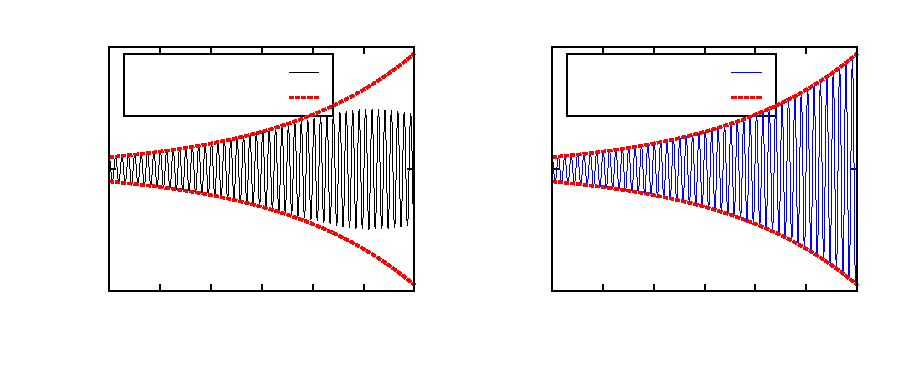
\includegraphics{swing_sim}}%
    \gplfronttext
  \end{picture}%
\endgroup
%}
\caption{Simulated swing angle, showing simulated results for both the
  original and the linearized ($\sin(\phi)\approx\phi_\text{lin}$)
  EOM. In these simulations $\epsilon=0.01$ and $a_0=0.1$. We see how the
  exponential growth becomes invalid for the original EOM after
  $t\approx400$, while the solution from the linearized EOM keeps on
  growing exponentially. 
}
\label{fig:sim}
\end{figure}


The equation of motion can of course also be solved numerically. The
numerical solutions are presented in \figref{fig:sim}; there we show
both the solution to the original EOM, \eqref{eq:eom}, and the
linearized version -- where $\sin(\phi)$ has been replaced by just
$\phi$. Then \figref{fig:sim_E} shows the energy of the solutions in
\figref{fig:sim}, as calculated using \eqref{eq:E}.

It is clear that the original EOM produces a solution which fits the
calculations, based on the linearized EOM, up to some amplitude. After
that amplitude the non-linear pendulum frequency-shift, due to an
amplitude dependent frequency, sets in and disrupts the
synchronization between the swing and the forcing. The synchronization is vital
to pump the swing with more energy, as can be seen in
\eqref{eq:DE_t0}. 

Furthermore when the phase of the swing and the
forcing is far enough apart the forcing will actually pump energy
\emph{out} of the swing, which can bee seen in \figref{fig:sim_E} at
$t\approx500$. If one continues on the numerical solution, one will
find that the amplitude of the swing will oscillate with a slow
frequency. This is because when the amplitude decreased, the
phase-shift will eventually drift back, and then the forcing
will again start pump energy into the swing. 

Meanwhile the linearized EOM yields a numerical solution that is
strikingly similar to what was predicted. This was to be expected
however, since the perturbation parameter $\epsilon=0.01$ in the
simulations is indeed $\ll1$.

\begin{figure}\centering
%\resizebox{.2\textwidth}{!}{
% GNUPLOT: LaTeX picture with Postscript
\begingroup
  \makeatletter
  \providecommand\color[2][]{%
    \GenericError{(gnuplot) \space\space\space\@spaces}{%
      Package color not loaded in conjunction with
      terminal option `colourtext'%
    }{See the gnuplot documentation for explanation.%
    }{Either use 'blacktext' in gnuplot or load the package
      color.sty in LaTeX.}%
    \renewcommand\color[2][]{}%
  }%
  \providecommand\includegraphics[2][]{%
    \GenericError{(gnuplot) \space\space\space\@spaces}{%
      Package graphicx or graphics not loaded%
    }{See the gnuplot documentation for explanation.%
    }{The gnuplot epslatex terminal needs graphicx.sty or graphics.sty.}%
    \renewcommand\includegraphics[2][]{}%
  }%
  \providecommand\rotatebox[2]{#2}%
  \@ifundefined{ifGPcolor}{%
    \newif\ifGPcolor
    \GPcolortrue
  }{}%
  \@ifundefined{ifGPblacktext}{%
    \newif\ifGPblacktext
    \GPblacktexttrue
  }{}%
  % define a \g@addto@macro without @ in the name:
  \let\gplgaddtomacro\g@addto@macro
  % define empty templates for all commands taking text:
  \gdef\gplbacktext{}%
  \gdef\gplfronttext{}%
  \makeatother
  \ifGPblacktext
    % no textcolor at all
    \def\colorrgb#1{}%
    \def\colorgray#1{}%
  \else
    % gray or color?
    \ifGPcolor
      \def\colorrgb#1{\color[rgb]{#1}}%
      \def\colorgray#1{\color[gray]{#1}}%
      \expandafter\def\csname LTw\endcsname{\color{white}}%
      \expandafter\def\csname LTb\endcsname{\color{black}}%
      \expandafter\def\csname LTa\endcsname{\color{black}}%
      \expandafter\def\csname LT0\endcsname{\color[rgb]{1,0,0}}%
      \expandafter\def\csname LT1\endcsname{\color[rgb]{0,1,0}}%
      \expandafter\def\csname LT2\endcsname{\color[rgb]{0,0,1}}%
      \expandafter\def\csname LT3\endcsname{\color[rgb]{1,0,1}}%
      \expandafter\def\csname LT4\endcsname{\color[rgb]{0,1,1}}%
      \expandafter\def\csname LT5\endcsname{\color[rgb]{1,1,0}}%
      \expandafter\def\csname LT6\endcsname{\color[rgb]{0,0,0}}%
      \expandafter\def\csname LT7\endcsname{\color[rgb]{1,0.3,0}}%
      \expandafter\def\csname LT8\endcsname{\color[rgb]{0.5,0.5,0.5}}%
    \else
      % gray
      \def\colorrgb#1{\color{black}}%
      \def\colorgray#1{\color[gray]{#1}}%
      \expandafter\def\csname LTw\endcsname{\color{white}}%
      \expandafter\def\csname LTb\endcsname{\color{black}}%
      \expandafter\def\csname LTa\endcsname{\color{black}}%
      \expandafter\def\csname LT0\endcsname{\color{black}}%
      \expandafter\def\csname LT1\endcsname{\color{black}}%
      \expandafter\def\csname LT2\endcsname{\color{black}}%
      \expandafter\def\csname LT3\endcsname{\color{black}}%
      \expandafter\def\csname LT4\endcsname{\color{black}}%
      \expandafter\def\csname LT5\endcsname{\color{black}}%
      \expandafter\def\csname LT6\endcsname{\color{black}}%
      \expandafter\def\csname LT7\endcsname{\color{black}}%
      \expandafter\def\csname LT8\endcsname{\color{black}}%
    \fi
  \fi
  \setlength{\unitlength}{0.0500bp}%
  \begin{picture}(6802.00,3400.00)%
    \gplgaddtomacro\gplbacktext{%
      \csname LTb\endcsname%
      \put(946,704){\makebox(0,0)[r]{\strut{}$10^{-3}$}}%
      \put(946,1873){\makebox(0,0)[r]{\strut{}$10^{-2}$}}%
      \put(946,3042){\makebox(0,0)[r]{\strut{}$10^{-1}$}}%
      \put(1078,484){\makebox(0,0){\strut{} 0}}%
      \put(1966,484){\makebox(0,0){\strut{} 100}}%
      \put(2854,484){\makebox(0,0){\strut{} 200}}%
      \put(3742,484){\makebox(0,0){\strut{} 300}}%
      \put(4629,484){\makebox(0,0){\strut{} 400}}%
      \put(5517,484){\makebox(0,0){\strut{} 500}}%
      \put(6405,484){\makebox(0,0){\strut{} 600}}%
      \put(176,1919){\rotatebox{-270}{\makebox(0,0){\strut{}$E(t)$}}}%
      \put(3741,154){\makebox(0,0){\strut{}$t$}}%
    }%
    \gplgaddtomacro\gplfronttext{%
      \csname LTb\endcsname%
      \put(2530,2907){\makebox(0,0)[r]{\strut{}$\phi(t)$}}%
      \csname LTb\endcsname%
      \put(2530,2687){\makebox(0,0)[r]{\strut{}$\phi_\text{lin}(t)$}}%
      \csname LTb\endcsname%
      \put(2530,2467){\makebox(0,0)[r]{\strut{}$E_0\exp(3\epsilon{t}/4)$}}%
    }%
    \gplbacktext
    \put(0,0){\includegraphics{swing_sim_energy}}%
    \gplfronttext
  \end{picture}%
\endgroup
%}
\caption{Energy, calculated using \eqref{eq:E}, of numerical solutions
  to both the original EOM ($\phi$) and the linearized
  ($\sin(\phi)\approx\phi_\text{lin}$), together with the calculated energy
  \eqref{eq:E(t)}. Note here that the energy from the linearized EOM
  and the approximated energy, \eqref{eq:E(t)}, is nearly
  indistinguishable in this figure.
}
\label{fig:sim_E}
\end{figure}



%  LocalWords:  parametrically EOM dimensionalize dimensionalized
%  LocalWords:  dimenzionalizing Floquet linearities rederive DEs
%  LocalWords:  Falk





%%% Local Variables: 
%%% mode: latex
%%% TeX-master: "Report_swing_circadian"
%%% End: 




\section{Introduction to Floquet Theory}
In the previous sections we showed that, in the linear approximation, a
swing with periodically varying length has solutions whose amplitude
increases or decreases exponentially in time. Although we didn’t show
this, there are also solutions that show no steady change in amplitude
with time. Which type of solutions one gets depends on the ratio of
the frequency $\omega$ of the length oscillation to the free-running
frequency $\omega_0$ of the unperturbed swing, and also on the magnitude  of the
length oscillation. As a general rule, exponential growth occurs when
the forcing entrains the oscillation of the swing in such a way that
the motions that deliver energy occur at the most effective phase of
each cycle. This is more likely to happen if the ratio $\omega/\omega_0$ is an integer
(as we showed, 2 is particularly effective), and when $\epsilon$ is larger.  

Floquet Theory is a general approach to understanding systems of
linear ODEs with periodic parametric forcing. Specifically, it applies
to systems of the form 
\begin{equation}\label{eq:floquetsys}%1
\dv{\vb{x}}{t}=\vb{A}(t)\vb{x}(t)
\qcomma \vb{x}(t_0)=:\vb{x}_0,
\end{equation}
where the matrix $\vb{A}(t)$ is a $T$-periodic function of time: 
\begin{equation}\label{eq:2}
\vb{A}(t+nT)=\vb{A}(t)\qcomma
n\in\Z.
\end{equation}
Every solution of \eqref{eq:floquetsys} is encompassed in its principal
fundamental matrix solution $\vb{U}(t,t_0)$, defined as the solution
to the matrix IVP  
\begin{equation}
\dv{\vb{U}(t,t_0)}{t}=\vb{A}(t)\vb{U}(t,t_0)\qcomma
\vb{U}(t_0,t_0)=\I
\end{equation}
Here  $\I$ is the  $n\times n$ identity matrix. Specifically, the
solution of \eqref{eq:floquetsys} is  $\vb{x}\left(t\right)=\vb{U}\left(t,{t}_{0}\right){x}_{0}$.

\bigskip
\noindent
Define the monodromy matrix $\vb{B}=\vb{U}({t}_{0}+T,{t}_{0})$. The monodromy
matrix turns out to be independent of  ${t}_{0}$, so it can be
computed as  $\vb{B}={U}(T,0)$. The eigenvalues of  $\vb{B}$,  $\rho_{1},\rho_{2},{\dots},\rho_{n}$, are called the characteristic
multipliers. The determinant of  $\vb{B}$ (the product of the
characteristic multipliers) is given by, 
\begin{equation}
\det(\vb{B})=\exp \left(
\int_{0}^{T}{\tr[\vb{A}(s)]\id{s}}
\right)
\end{equation}
The multipliers determine the character (e.g. stable or exponentially
growing) of solutions of \eqref{eq:floquetsys}. In particular, 
\begin{equation}
\vb{U}(t,{t}_{0})=
\vb{U}\Big((t-{t}_{0})\;\;\text{mod} T,\,{t}_{0}\Big)
{\vb{B}}^{\lfloor(t-{t}_{0})/T\rfloor}
\end{equation}

The characteristic exponents  
$\mu_{1},\mu_{2},{\ldots},\mu_{n}$, defined by  $\ee^{\mu_{i}T}=\rho_{i}$ determine the
growth rate of solutions. In particular, if  $\Re(\mu_{i})<0$,
solutions associated with it will decay exponentially; if
$\Re(\mu_{i})>0$, solutions associated with it will grow
exponentially, and if  $\Re(\mu_{i})=0$, solutions 
associated with it will be stable. (Strictly speaking, the previous
statements hold only if the geometric multiplicity of each eigenvalue
of  $\vb{B}$ equals its algebraic multiplicity. When this is not the case,
polynomial factors can also arise.) There will be, associated with
each characteristic exponent  $\mu$, a solution of the form 
\begin{equation}
\vb{x}(t)=\ee^{\mathit{\mu t}}\vb{p}(t)
\end{equation}
where  $\vb{p}(t)$ is a  $T$-periodic vector function of time. 

A particularly interesting case arises when  $\vb{A}(t)$ is a periodic
perturbation of a constant matrix that itself has 
${T}_{0}${}-periodic solutions, i.e.
\begin{equation}
\vb{A}(t)={\vb{A}}_{0}+\epsilon \widetilde{{\vb{A}}}(t)
\end{equation}
with  $\widetilde{{\vb{A}}}(t)$  $T${}-periodic. For instance, the varying
length swing is of this form, with
\begin{equation}
\begin{aligned}
\vb{A}_0&=
\begin{pmatrix}0&1\\-{\eta }^{2}&0\end{pmatrix}
\\
\widetilde{{\vb{A}}}(\tau)&=
\begin{pmatrix}0&0\\
0&-2\frac{\dot{{r}}(\tau)}{r(\tau)}
\end{pmatrix}
=
\begin{pmatrix}0&0\\
0&-2\pd_{\tau}\log(r(\tau))
\end{pmatrix}.
\end{aligned}
\end{equation}
${\vb{A}}_{0}$ is traceless, and since  $r$ is periodic, the integral of 
$\tr(\widetilde{{\vb{A}}})$ over one cycle is  
$-2\log({\tau}_{0}+2\pi )+2\log({\tau }_{0})=0$. Thus the
monodromy matrix  $\vb{B}$ for the swing has determinant 0. The character
of the solutions can be determined from  $\tr(\vb{B})$.
If  $\abs{\rho_{1}+\rho_{2}}=|\tr(\vb{B})|<2$, the multipliers  
$\rho_{1},\rho_{2}$ form a complex conjugate pair, each with absolute
value 1, and solutions are stable. If, however,
$\abs{\rho_{1}+\rho_{2}}=|\tr(\vb{B})|>2$, the multipliers
are real and different, and since their product is 1, one must be
greater than one. In this case, there is an exponentially growing
solution. Finally, in the border case,  $|\rho_{1}+\rho_{2}|=\tr(\vb{B})=2$, the multipliers are equal
, either both 1 or both  $-1$. The values of  $\eta,\,\epsilon $ for
which that holds define the boundaries of the Floquet tongues, within
which exponentially growing solutions occur. 





%%% Local Variables: 
%%% mode: latex
%%% TeX-master: "Report_swing_circadian"
%%% End: 




\section{Circadian rhythms}
Every human being, and indeed many or most living things, contains at
least one internal clock (Ko and Takahashi,~2006; Partch et al.,~2014;
Rosato et al., 2006). Biological clocks with a period of 
approximately 24 hours are called \textit{circadian} clocks (meaning
“about a day”). The consequences of an incorrectly working clock
become obvious when one flies from Canada to Japan.

The circadian clock is a chemical limit cycle oscillator. Ronald
Konopka and Seymour Benzer~(1971), working in the fruit fly
\textit{Drosophila melanogaster} discovered a gene \textit{period}
(\textit{per}), that affects the period of the fly's circadian clock.
We now know that \textit{per} is a central component of the clock.
The clock works by negative feedback with delay. \textit{per}
contains the information for making a protein, called PER. To make
PER protein, the \textit{per} gene must be transcribed to produce a
messenger RNA (mRNA), which is translated into PER protein in the
cytoplasm (that part of the cell outside the nucleus). The PER
protein then moves into the nucleus (where the genes are) and
represses transcription of the \textit{per} gene. 

\subsection{An ODE model of a circadian oscillator}
A minimal circadian clock model has three ODEs describing the dynamics
of PER mRNA, cytoplasmic PER protein, and nuclear PER protein (Pfeuty
et al., 2011). This three ODE model, which we will use, is as
follows,
\begin{equation}\label{eq:Pfeutysystem}
\begin{aligned}
\tau\dv{M}{t}&={s}_{M}\frac{{K}_{I}^{n}}{{K}_{I}^{n}+\PN^{n}}-{d}_{M}\frac{M}{{K}_{M}+M}\\
\tau\dv{\PC}{t}&={s}_{P}M-{d}_{P}\frac{\PC}{{K}_{P}+\PC}-{k}_{1}\PC+{k}_{2}\PN\\
\tau \dv{\PN}{t}&={k}_{1}\PC-{k}_{2}\PN
\end{aligned}
\end{equation}
Here  $M$ is concentration of \textit{per} mRNA, and  $\PC$ and 
$\PN$ the concentrations of PER protein in the cytoplasm and
nucleus. The first equation describes the synthesis and degradation
of the mRNA. Synthesis occurs at rate  ${s}_{M}$ in the absence of
nuclear PER, but is inhibited by PER. Degradation follows standard
Michaelis-Menten kinetics. In the second equation we see that
cytoplasmic PER protein is made at a rate that depends on the mRNA
concentration and is degraded. The final two terms of the second
equation and both terms of the third describe exchange of PER protein
between cytoplasm and nucleus. 

With dark parameter values  $n=4$,  ${s}_{M}=2.2$,  ${K}_{I}=1.8$, 
${d}_{M}=0.84$,  ${K}_{M}=0.5$,  ${s}_{P}=0.4$,  ${d}_{P}=1.6$, 
${k}_{P}=0.13$,  ${k}_{1}=0.4$,  ${k}_{2}=0.45$,  $\tau =1$ the
free-running period becomes  ${T}_{0}{\approx}\unit[24]{h}$. This system is
easily solved numerically (Figure 1). 

\subsection{Entrainment: setting the clock}
The clock is not useful unless it can be set. Real circadian clocks
are quite inaccurate, with typical free-running periods of about
25.5\,h, so they need to be set daily. In practice, environmental
light levels affect the parameters of the differential equations \eqref{eq:Pfeutysystem} in
such a way as to establish a consistent relationship with the
day/night cycle. This process is called entrainment. Our next goal is
to understand how entrainment occurs. 

\subsection{Dimensional reduction: phase}
To analyze this system, we simplify it from three dimensions to one by
focusing on the limit cycle  $C$. Our goal is to assign to every
point  $(M,\PC,\PN)$ near  $C$ a phase  $\phi{\in}\R/{T}_{0}\Z$
(${T}_{0}$ is the free-running period of the clock), and then to study
the evolution of this scalar function of time. 

Begin by writing the ODE system in generic form
\eqref{eq:IVP}. ($\vb{x}=(M,\PC,\PN)$ and $\vb{p}$ is the parameter vector
$(n,{S}_{M},{\dots},{k}_{1},{k}_{2})$.  
\begin{equation}\label{eq:IVP}
\dv{\vb{x}}{t}=\vb{F}(\vb{x};p)
\vb{x}(0)={\vb{x}}_{0}
\end{equation}

Now define  $\vb{x}({\vb{x}}_{0},t)$ as the solution to the autonomous system
\eqref{eq:IVP}. We assign phase 0 to some arbitrary point in  $C$, then define 
$\phi$ at other locations by 
\begin{equation}\label{eq:phidef}
\phi (\vb{x}({\vb{x}}_{0},t))=\phi
({\vb{x}}_{0})+t
\end{equation}
That is, phase always advances by one hour for every hour that passes.
(Later, when we have external periodic forcing, we will scale 
$\phi$ so that its period is different from  ${T}_{0}$.) \eqref{eq:phidef} is
sufficient to define  $\phi$ on  $C$ (up to the choice of zero).
To define  $\phi$ outside  $C$, we require  $\phi(\vb{x})$ to be
continuous and differentiable. The limit cycle is attractive. If you
start anywhere in its basin of attraction, you will eventually
approach the cycle arbitrarily closely. At that point  $\phi(\vb{x})$
must, by continuity, be close to the phase of the nearest point in 
$C$.  $\phi(\vb{x})$ is therefore approximately defined, and by
extrapolation,  $\phi$ is approximately defined at every point on
the trajectory that led to  $\vb{x}$. To first order,  $\phi$ near 
$C$ is defined by the gradient of  $\phi$ on  $C$, as follows. 

Choose a point  ${\vb{x}}_{C}{\in}C$ with
$\phi({\vb{x}}_{C})={\phi}_{C}$, and call the gradient of  $\phi$
there  ${\nabla}\phi({\vb{x}}_{C})$. Let  $\vb{u}$ be a unit vector, and
$|\epsilon|{\ll}1$. Define
${\vb{x}}_{1}={\vb{x}}_{C}+\epsilon\vb{u}$. Then  
\begin{equation}
\phi ({\vb{x}}_{1})=\phi({\vb{x}}_{C}+\epsilon\vb{u})
=\phi({\vb{x}}_{C}) + \epsilon{\vb{u}}^{\T}\,{\nabla}\phi
({\vb{x}}_{C})+O({\epsilon }^{2})
\end{equation}
Now, project both  $\vb{x}_{C}$ and  $\vb{x}_{1}$ forward in time by 
$0<\delta\ll1$, to new points  $\vb{x}_{C\delta}$ and 
$\vb{x}_{1\delta}$. 
\begin{equation}\label{eq:xdelta}
\begin{aligned}
{\vb{x}}_{C}\to& \vb{x}_{C\delta}
=\vb{x}_{C}+\delta\vb{F}({\vb{x}}_{C})+\order{\delta^2},\\
\phi({\vb{x}}_{\mathit{C\delta }})=&{\phi}_{C}+\delta. \\
\vb{x}_1\to& \vb{x}_{1\delta}
 =\vb{x}_{C}+\epsilon \vb{u}+
  \delta\qty[\vb{F}(\vb{x}_{C})+\epsilon \vb{J}(\vb{x}_{C})\vb{u}
  +\order{\epsilon^2}],\\
\phi({x}_{1\delta })=&\phi(\vb{x}_{C}) + \delta 
 +\epsilon {\vb{u}}^{\T}\,{\nabla}\phi(\vb{x}_{C})
 +\order{\epsilon^2}.
\end{aligned}
\end{equation}
We used that the flow at  $\vb{x}_{1}$ is 
$\vb{F}(\vb{x}_{1})
=\vb{F}(\vb{x}_{C}+\epsilon\vb{u})
=\vb{F}(\vb{x}_{C})+\epsilon\vb{J}(\vb{x}_{C})\vb{u}+\order{\epsilon^2}$, where 
$\vb{J}(\vb{x}_{C})={\nabla}\vb{F}(\vb{x}_{C})$ is the Jacobian of the
flow field at  $\vb{x}_{C}$. Now, we're in position to find the gradient
at the new location, using
\begin{equation}
\phi(\vb{x}_{1\delta })-\phi(\vb{x}_{C\delta})
=(\vb{x}_{1\delta }-\vb{x}_{C\delta})^{\T}\,
{\nabla}\phi(\vb{x}_{C\delta})+\order{\epsilon^2}.
\end{equation}
Plugging in \eqref{eq:xdelta} and equating terms of  $\order{\epsilon}$ 
(details fell casualty to the page limit) gives
\begin{equation}\label{eq:ueq}
\epsilon {\vb{u}}^{\T}\,{\nabla}\phi(\vb{x}_{C})=\epsilon
{\vb{u}}^{\T}\,\qty(\I+\delta\vb{J}(\vb{x}_{C})^{\T})
{\nabla}\phi(\vb{x}_{C\delta})
\end{equation}
$\I$ is the identity matrix. Now remember, $\vb{u}$ is an
arbitrary unit vector, and \eqref{eq:ueq} must be true for all  $\epsilon\vb{u}$. This
is possible only if the vector  ${\vb{u}}^{\T}$ is multiplied by is the
same on both sides. Since  $\delta\ll1$,  
$(\I+\delta\vb{J}(\vb{x}_{C})^{\T})^{-1}
=(\I-\delta\vb{J}(\vb{x}_{C})^{\T})+\order{\delta^2}$. 
Thus, to $\order{\delta}$,
\begin{equation}
\begin{aligned}
{\nabla}\phi(\vb{x}_{C})&=\qty(\I+\delta\vb{J}{(\vb{x}_{C})}^{\T})
{\nabla}\phi(\vb{x}_{C\delta})\\
\qty(\I-\delta \vb{J}(\vb{x}_{C})^{\T})
{\nabla}\phi(\vb{x}_{C})&={\nabla}\phi(\vb{x}_{C\delta})\\
\frac{{\nabla}\phi(\vb{x}_{C\delta})-{\nabla}\phi(\vb{x}_{C})}{\delta}
&=-\vb{J}{(\vb{x}_{C})}^{\T}\,{\nabla}\phi(\vb{x}_{C})
\end{aligned}
\end{equation}
The final line is a first-order approximation to 
$\dv{t} \nabla\phi(x(t))$. Thus, we end up at last with 
\begin{equation}\label{eq:gradphiODE}
\dv{t} \nabla\phi(x)
=-\vb{J}(x)^{\T}\,\nabla\phi(x)
\end{equation}
valid in  $C$. Other than complexity, there is no obvious obstacle to
continuing this analysis to higher order, but we have not done so. 

We now have a linear ODE in ${\nabla}\phi$. We need only an
initial condition. 

Remember that  $\vb{x}(t)$ circulates around  $C$ at a rate that we have
determined (analytically or numerically), so  $\vb{J}(x)$ can just as well
be written  $\vb{J}(t)$. Thus \eqref{eq:gradphiODE} is a periodic nonautonomous linear
system of ODEs in  ${\nabla}\phi$. As described above, this
system has a general solution that can be expressed as a power of its
monodromy matrix times a periodic function of time. That is, its
principal fundamental solution matrix  $\vb{U}(t,0)$ can be written as 
\begin{equation}
\vb{U}(t,0)=\vb{U}(t\;\;\text{mod}{T}_{0},\,0)\vb{B}^{\lfloor t/{T}_0\rfloor}
\end{equation}
Vector  ${\nabla}\phi(t)=\vb{U}(t, 0){\nabla}\phi(0)$ 
is a solution to \eqref{eq:gradphiODE}. ${\nabla}\phi$ must be a periodic function of
time on $C$. In particular, 
\begin{equation}
\nabla\phi(T_0)=\vb{B}\,\nabla\phi(0)={\nabla}\phi(0)
\end{equation}
That is,  ${\nabla}\phi(0)$ must be an eigenvector of
the monodromy matrix with eigenvalue 1, i.e. 1 must be a
characteristic multiplier. Indeed, there is a straightforward
argument that it is (Ward). 





\subsection{Phase response curves}
Light does not directly affect  $\vb{x}=(M,\PC,{P}_{M})$ --- it affects the
parameters of the differential equations \eqref{eq:Pfeutysystem}. We now suppose that the
parameter vector  $\vb{p}$ varies with time,
\begin{equation}
\vb{p}=\vb{p}_{0}+\mathit{\epsilon L}(t)\vb{dp}.
\end{equation}
The effect vector  $\vb{dp}$ is of order of magnitude 1 giving the
direction of the parameter changes induced by light. The light function 
$L(t)$ is normalized so as to be order of magnitude 1 and specifies
how light varies over the course of a day --- e.g. 12\,h on, 12\,h off. It
is periodic with period  $T$. We scale the phase defined by \eqref{eq:phidef} so
that, instead of running from 0 to  ${T}_{0}$, it runs from 0 to 
$T$. Now, let  ${\phi}_{n}$ be the phase at dawn on day  $n$.
Then, in constant darkness,
\begin{equation}
\phi_{n+1}=\phi_{n}-\gamma.
\end{equation}
$\gamma$ is a measure of the difference between  ${T}_{0}$ and  $T$.
For instance, with  $T=24$, ${T}_{0}=25$, $\gamma =0.96$ --- the clock
loses a little less than an hour a day in the darkness. Now, what
happens if we turn on the lights, i.e. allow  $\epsilon\neq0$? The
dawn-to-dawn effect on phase depends on the phase of the clock at
dawn. It is given by the phase response curve (PRC),  $V(\phi)$,
defined by 
\begin{equation}
\phi_{n+1}=\phi_{n}-\gamma +V(\phi_{n}).
\end{equation}
The PRC $V(\phi)$ intrinsically depends on  $\epsilon$,  $L(t)$, and
$\vb{p}_{0}$ and  $\vb{dp}$. This difference equation has a fixed
point  ${\phi}^{?}$ if  $V({\phi}^{?})=\gamma $.
This fixed point is stable if  
$-2<\dv{V(\phi^{*})}{\phi}<0$. 
Because of its importance to stability, Pfeuty et al (2011) give 
$\dv{V(\phi^{*})}{\phi}$ a name:~$\chi$. 
Thus, we expect entrainment if two conditions are met: the PRC attains
the value  $\gamma$ for some  $\phi$, and  $-2<\chi<0$. 


\bigskip
We have everything we need to calculate the PRC. Phase changes as
follows, 
\begin{equation}
\begin{aligned}
\dv{\phi}{t}&=1+\epsilon\,L(\phi)\,Z(\phi)+\order{\epsilon^2}
\\
Z(\phi)&={({\nabla}\phi(\phi))}^{\T}\,
\qty(\pdv{\vb{F}(\vb{x}(\phi),\, \vb{p}_{0})}{\vb{p}})\vb{dp}
\end{aligned}
\end{equation}
$Z(\phi)$ (Figure 2B) is called the infinitesimal impulse phase
response curve (IPRC) and gives the response of phase to an
infinitesimal delta-function light stimulus at phase  $\phi$. The
PRC is calculating by convolving  $Z(\phi)$ with  $L(t)$

\begin{equation}\label{eq:convolution}
\begin{aligned}
V(\phi)&=\epsilon \int_{0}^{T}\! 
L(u)Z\qty(u\frac{T}{{T}_{0}}+\phi) \id{u}
\\
&\approx\epsilon \int_{0}^{T}\!
L(u)Z(u+\phi)\id{u}
\\
&=\epsilon \int _{0}^{\tau_\text{D}}\!
L(u)Z(u+\phi)\id{u}
\end{aligned}
\end{equation}
The approximation in the second step is valid if  $\gamma\ll1$. The
final version holds in the common situation in which light is only
available during ``daytime'', defined as the period from dawn ($t=0$)
until sunset  $(t=\tau_\text{D}$), so that  $L(u)=0$ outside
 $[0,\;\tau_\text{D}]$. 





\subsection{Robustness}
The PRC and the IPRC are products of evolutionary design. Both the
effect of light on the parameter values,  $\vb{dp}$, and the
magnitude of that effect,  $\epsilon $, are the result of
evolutionary pressures. A minimal criterion for a working clock is
that it should be stably entrained by the light cycle, and the
previous section described the mathematical requirements to
accomplish that goal. But there's more: In real life, the light curve
 $L(u)$ is variable. It varies because of the season, the weather,
and the behavior of the animal. A well-working circadian clock should
not be excessively sensitive to such variations. Variations in the
light curve are modeled as perturbations of  $L(u)$:
\begin{equation}
\epsilon\,L(u)
=\epsilon_{0}\qty({L}_{0}(u)+\eta \widetilde{{L}}(u)),
\end{equation}
where ${L}_{0}$ and  $\widetilde{{L}}$ are normalized to order of magnitude
1, and  $\eta$ is small compared to 1. $\phi^{*}$ and $\chi$ are now
functions of $\eta$. Robustness requires that they not be excessively
sensitive to  $\eta$.

Pfeuty et al (2011) develop two measures of robustness,

\begin{equation}
\begin{aligned}
\varPi &=\eval{\qty(\dv{\eta} \phi^{*}(\eta) )^{2}}_{\eta=0}
\\
\varSigma &=\eval{\qty(\frac{1}{\chi(\eta)}
\dv{\eta} \chi(\eta) )^{2}}_{\eta=0}
\end{aligned}
\end{equation}
To estimate these, we begin with the PRC
\begin{equation}\label{eq:Vtilde}
V(\phi)=V_{0}(\phi)
+\eta\widetilde{V}(\phi)
\end{equation}
$V_{0}$ and $\widetilde{V}$ are the convolutions of the IPRC 
$Z$ with $\epsilon_{0}L_{0}$ and 
$\epsilon_{0}\widetilde{L}$ according to \eqref{eq:convolution}. Now, 
$V({\phi}^{*}(\eta))=\gamma$ is constant. Thus, expanding
\eqref{eq:Vtilde} around $\phi^{*}(0)$, 
\begin{equation}
\eta \qty(\widetilde{V}\Big(\phi^{*}(0)\Big)
+{V}_{0}'\Big(\phi^*(0)\Big)\dv{\phi^{*}(0)}{\eta})
+\order{\eta^2} = 0
\end{equation}
Neglecting $\order{\eta^2}$ terms, we can solve for an estimate of
robustness measure $\varPi$,
\begin{equation}
\varPi=\qty(
\frac{\widetilde{V}(\phi_{0}^{*})}
{\widetilde{V}'(\phi_{0}^{*})}
)^{2}
\end{equation}
where $\phi_{0}^{*}\equiv\phi^{*}(0)$. By similarly
expanding $\chi(0)$, we obtain an estimate of $\varSigma$,
\begin{equation}
\varSigma =\qty(
\frac{\widetilde{V}'(\phi_0^{*})}
{V_0'(\phi_0^{*})}
-\frac{\widetilde{V}(\phi_0^{*}){V}_0''(\phi_0^{*})}
{V_0'(\phi_0^{*})^{2}}
)^{2}
\end{equation}
Pfeuty et al (2011) show using these measures that some IPRCs give
rise to more robust PRCs than others. In particular, the main
characteristics of a robust IPRC are that it possess a “dead zone”
that cover most of the day time (this makes the PRC insensitive to
variations in the daytime light profile), and that it have sharply
negative slope near the beginning and end of the night. 

A great advantage of the PRC and IPRC as ways of characterizing
circadian clocks is that they can be directly measured. Pfeuty et al
(2011) cull a dozen IPRCs from the literature, and show that they are
indeed robust. 






















%%%%%%%%%%%%%%%%%%%%%%%%%%%%%%%%%%%%%%%%%%%%%%%%%%%%%%%%%%%%%%%%%%%%%%%%%%%%%%%%
\begin{comment}

\section{Figures}

\begin{flushleft}
\tablehead{}
\begin{supertabular}{|m{2.99626in}m{2.99696in}|}
\hline
\multicolumn{1}{|m{2.99626in}|}{A.

\centering 
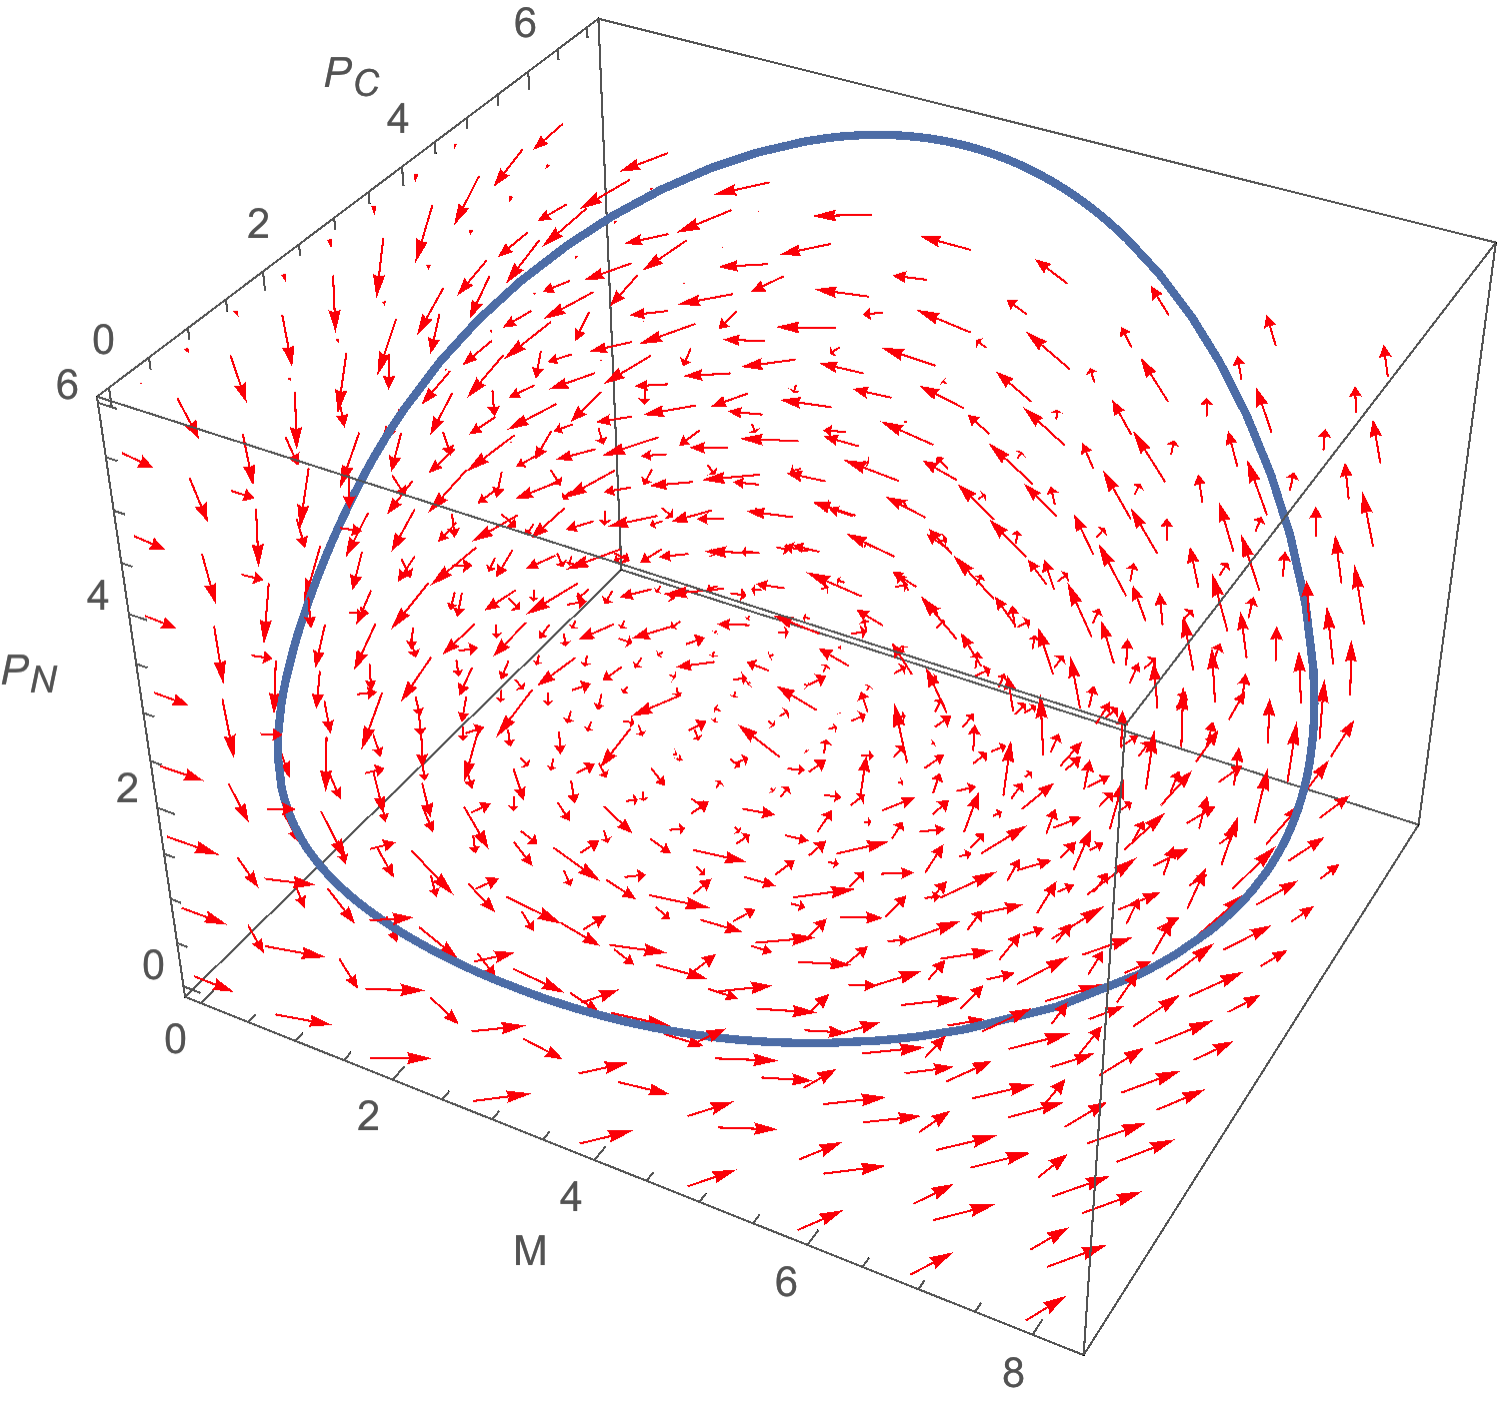
\includegraphics[width=3.5in,height=3.2862in]{reportv7-img1.png} } &
B.

\centering\arraybslash 
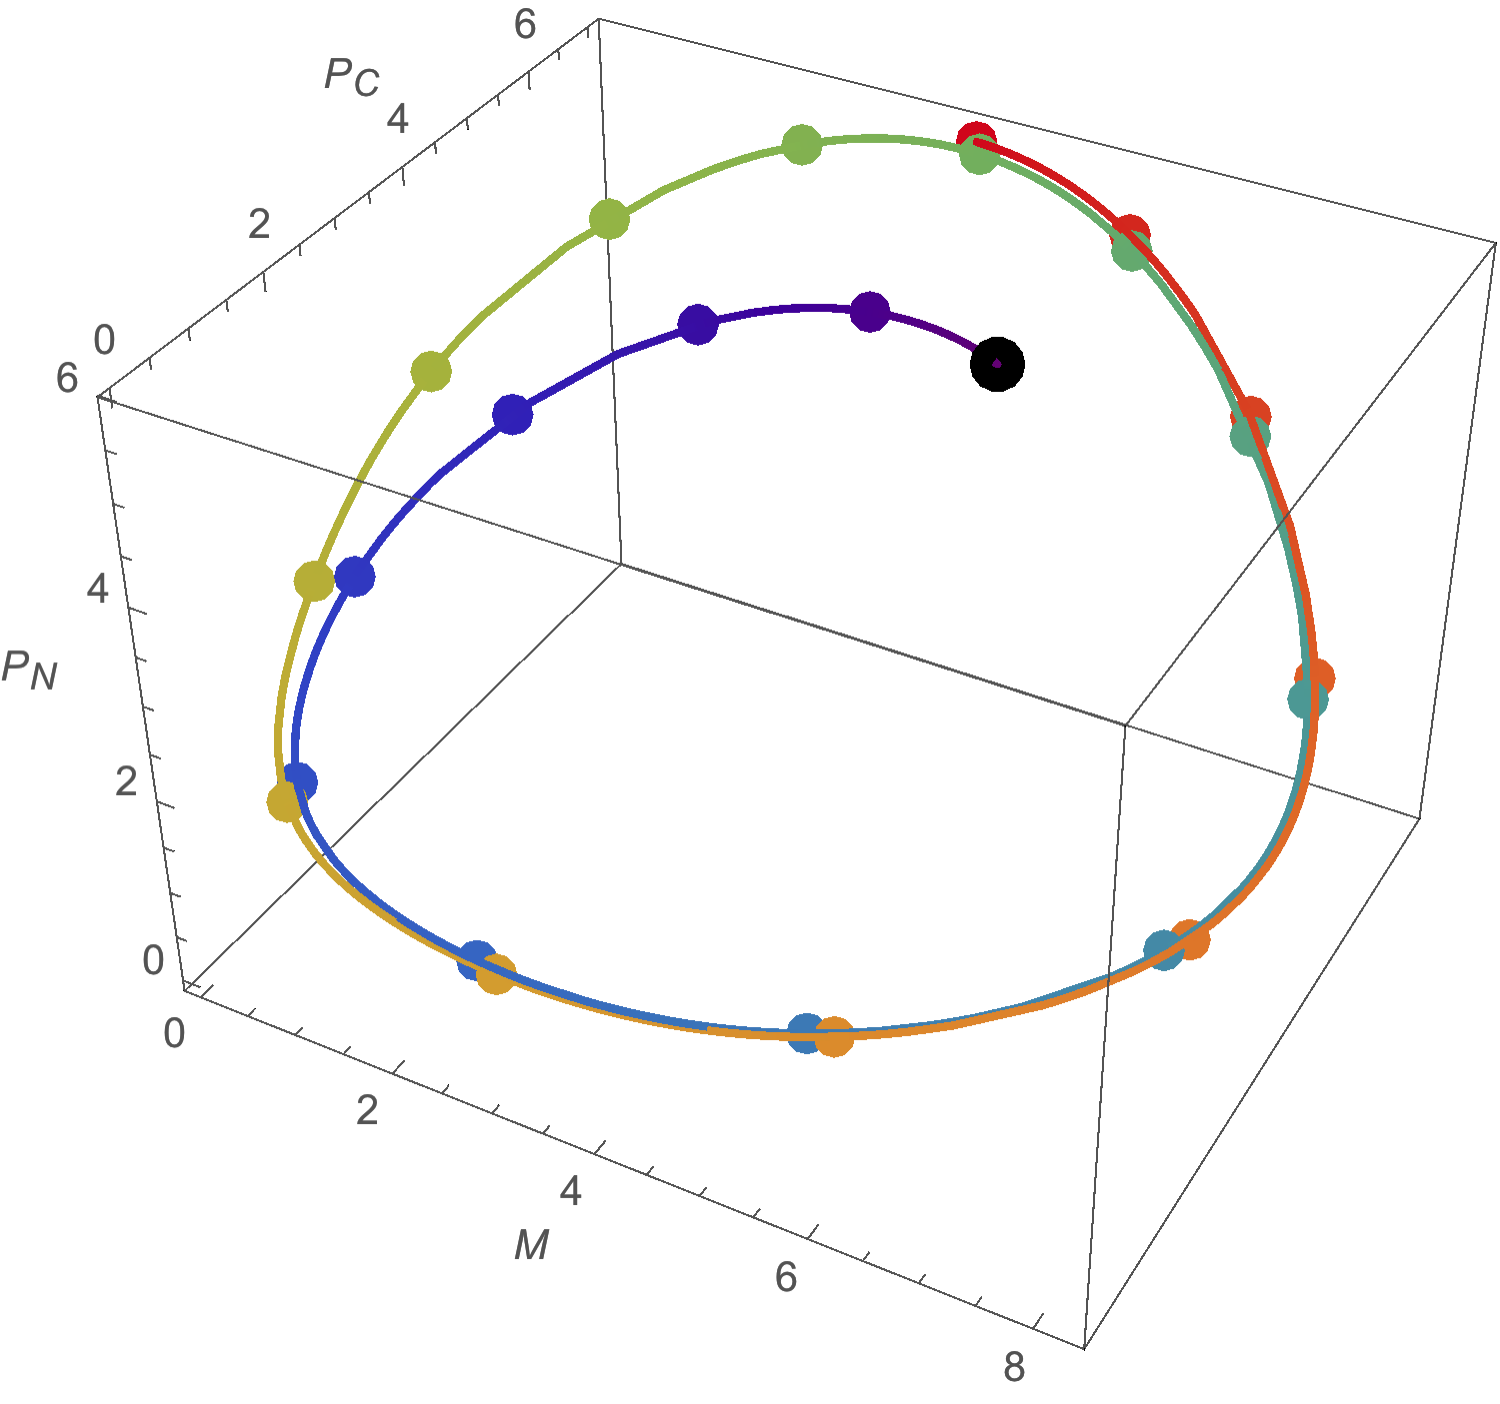
\includegraphics[width=3.5in,height=3.2764in]{reportv7-img2.png}
\\\hline
\multicolumn{2}{|m{6.07196in}|}{{\bfseries
\label{eq:Ref341089568}Figure \stepcounter{Figure}{\theFigure}:
Numerical solution of the ODE model}

A. Flow vector field corresponding to the system \eqref{eq:Pfeutysystem}. Flow vectors are
shown in red, the limit cycle $C$ in blue. B. Numerical solution for
48h starting from a randomly chosen point (black), showing
convergence to $C$. Colored dots are placed every two hours, with
color changing from purple to red with the passage of time. }\\\hline
\end{supertabular}
\end{flushleft}

\bigskip

\begin{center}
\tablehead{}
\begin{supertabular}{|m{2.99626in}|m{2.99696in}|}
\hline
A. ${\nabla}\phi(\phi)$

 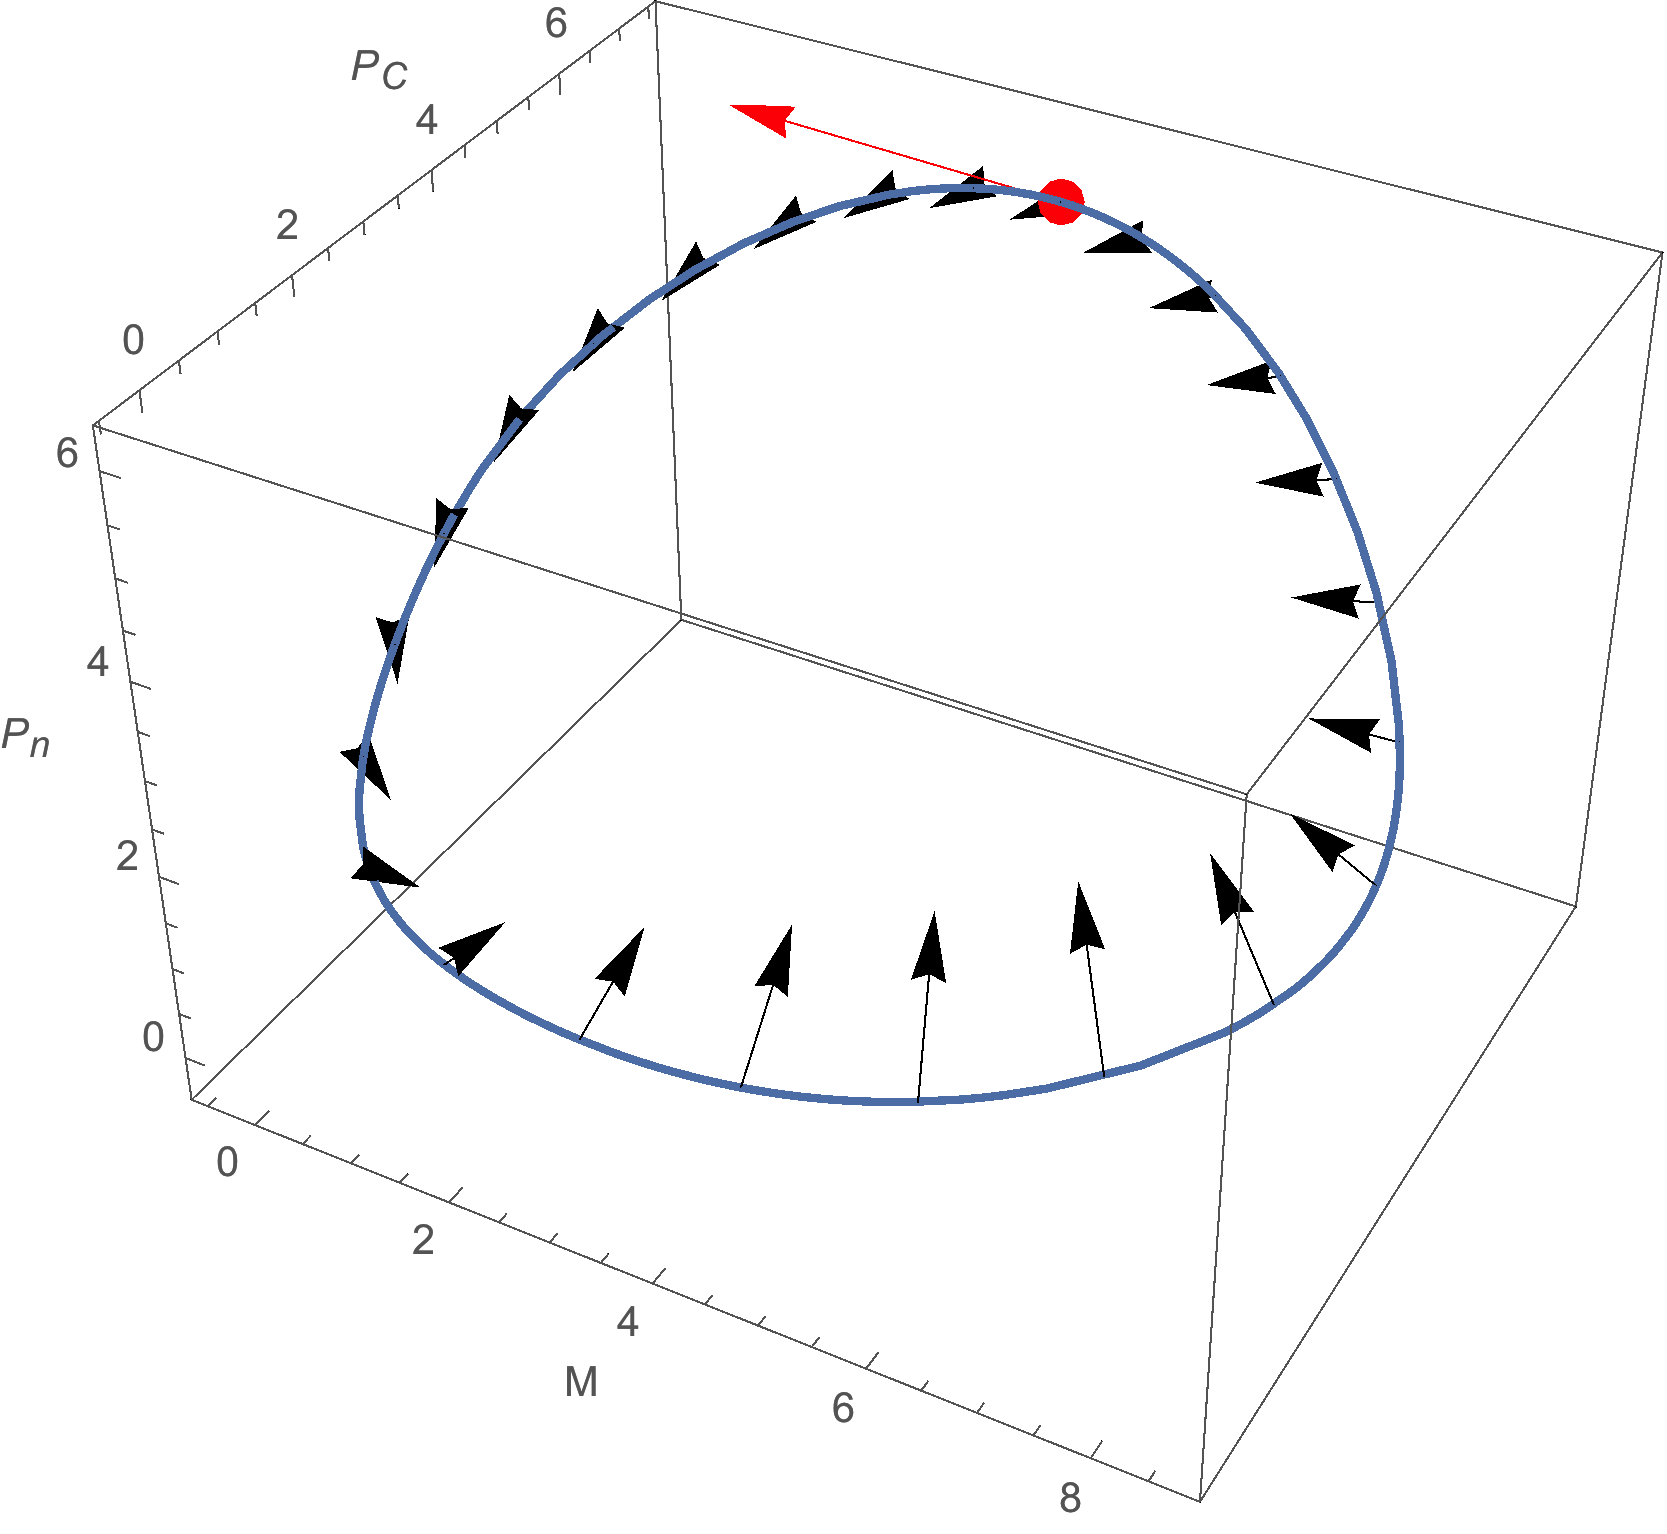
\includegraphics[width=3.5in,height=3.2193in]{reportv7-img3.png} 

~
 &
B. $Z(\phi)$

  [Warning: Image ignored] % Unhandled or unsupported graphics:
%\includegraphics[width=3.5in,height=2.1in]{reportv7-img4}
 \\\hline
 &
C. $V(\phi)$

  [Warning: Image ignored] % Unhandled or unsupported graphics:
%\includegraphics[width=3.5in,height=2.1346in]{reportv7-img5}
 \\\hline
\multicolumn{2}{|m{6.07196in}|}{{\bfseries
\label{eq:Ref341096105}Figure \stepcounter{Figure}{\theFigure}: 
${\nabla}\phi$ for the Pfeuty et al (2011) system.}

A. In blue is the limit cycle. The red arrow shows the direction of
progress around the cycle. The 24 black arrows show numerically
computed phase gradients at each hour around the cycle. B. The
corresponding IPRC, computed using $\vb{dp}$ being a change of 
$-1$ in parameter ${S}_{M}$. \ The gray bar corresponds to daytime 
$t{\in}[0,12]$, based on the resulting PRC in part C. This panel
approximately reproduces the left-hand panel of Pfeuty et al (2011),
Figure 3A. C. The corresponding PRC with $\epsilon =0.3$, 
$L(t)=\{\begin{matrix}2\text{ if
}0{\leq}t<12\\0\text{ if }12{\leq}t<24\end{matrix}\}$. With 
$\gamma =0.96$, there is a stable fixed point $\phi^{*}=16.66,\chi =-0.799$. This figure approximately reproduces the
left-hand panel of Pfeuty et al (2011), Figure 2A.}\\\hline
\end{supertabular}
\end{center}

\bigskip


\bigskip

\begin{flushleft}
\tablehead{}
\begin{supertabular}{|m{3.49346in}|m{3.3490598in}|}
\hline
  [Warning: Image ignored] % Unhandled or unsupported graphics:
%\includegraphics[width=3.5in,height=3.7972in]{reportv7-img6}
  &
{\bfseries Figure \stepcounter{Figure}{\theFigure}: Experimental IPRCs
show robustness characteristics}

This is a copy of Pfeuty et al (2011), Figure 5.

A. Experimentally measured IPRCs collected from the literature. B.
Estimated IPRCs from fitting the data in A. C. a-j: Estimated
robustness measure $\varPi}^{1/2}$ computed for experimental IPRCs in
B. m: range of$\varPi^{1/2}$ for all coupling schemes for the
computation al model. Horizontal line: $\varPi^{1/2}$ for an IPRC
that is linearly decreasing during daytime. \\\hline
\end{supertabular}
\end{flushleft}

\bigskip


\bigskip

\end{comment}
%%%%%%%%%%%%%%%%%%%%%%%%%%%%%%%%%%%%%%%%%%%%%%%%%%%%%%%%%%%%%%%%%%%%%%%%%%%%%%%%







%%% Local Variables: 
%%% mode: latex
%%% TeX-master: "Report_swing_circadian"
%%% End: 



\section*{Bibliography}
\noindent
Burns, J.A. (1970). \textit{More on Pumping a Swing}. Am. J. Phys. \textbf{38}, 920-2

\bigskip\noindent
Ko, C.H., and Takahashi, J.S. (2006). \textit{Molecular components of the
mammalian circadian clock}. Hum. Mol. Genet. R271-7.

\bigskip\noindent
Konopka, R.J., and Benzer, S. (1971). \textit{Clock Mutants of Drosophila
melanogaster}. \textbf{68}, 2112–2116.

\bigskip\noindent
Partch, C.L., Green, C.B., Takahashi (2014).
\textit{Molecular architecture of the mammalian circadian clock}. Trends Cell
Biol. \textbf{24}, 90–99.

\bigskip\noindent
Pfeuty, B., Thommen, Q., and Lefranc, M. (2011). \textit{Robust Entrainment of
Circadian Oscillators Requires Specific Phase Response Curves}.

\bigskip\noindent
Rosato, E., Tauber, E., and Kyriacou, C.P. (2006). \textit{Molecular genetics
of the fruit-fly circadian clock}. Eur. J. Hum. Genet. \textbf{14},
729–738.

\bigskip\noindent
Strub, D.C. (2009). \textit{How do children swing?}  M.Eng. thesis, University
of Bristol, Dept. of Eng. Math.%ematics

\bigskip\noindent
Tea, P.L. Jr. and Falk, H. (1968). \textit{Pumping on a Swing}. Am. J. Phys. 
\textbf{36}, 1165-6

\bigskip\noindent
Ward, M.J. \textit{Basic Floquet Theory}
(http://www.math.ubc.ca/\~{}ward/teaching/m605/every2\_floquet1.pdf).


\end{document}





%%% Local Variables: 
%%% mode: latex
%%% TeX-master: "Report_swing_circadian"
%%% End: 
